\newcommand{\distance}{4.6em}
\newcommand{\circlesize}{3.9em}
\newcommand{\imagesdistance}{3.8*\distance}

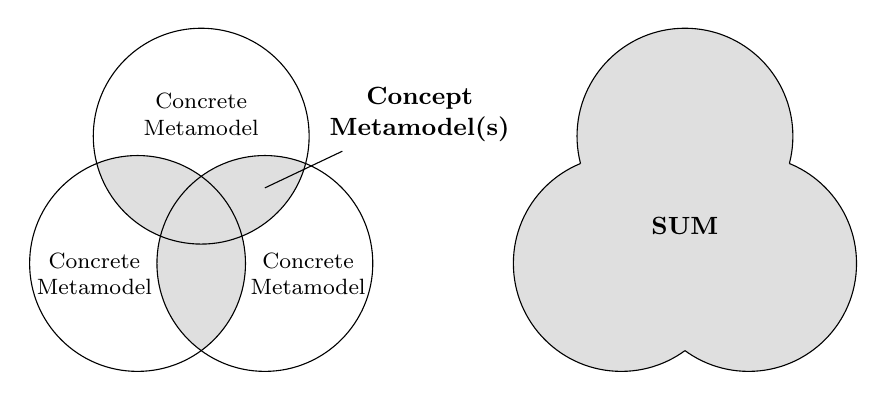
\begin{tikzpicture}[
    concrete font/.style={font=\footnotesize},
    concept font/.style={font=\small\bfseries},
    concept color/.style={lightgray!50}
]

% CONCEPTS
\def\concepta{(0,0) circle (\circlesize)}
\def\conceptb{(\distance,0) circle (\circlesize)}
\def\conceptc{(0.5*\distance,\distance) circle (\circlesize)}

% Filling
\begin{scope}
    \clip \conceptb;
    \fill[concept color] \concepta;
\end{scope}

\begin{scope}
    \clip \conceptc;
    \fill[concept color] \conceptb;
\end{scope}

\begin{scope}
    \clip \concepta;
    \fill[concept color] \conceptc;
\end{scope}

% Borders
\draw \concepta;
\draw \conceptb;
\draw \conceptc;


% SUM
\def\suma{(\imagesdistance,0) circle (\circlesize)}
\def\sumb{(\imagesdistance+\distance,0) circle (\circlesize)}
\def\sumc{(\imagesdistance+0.5*\distance,\distance) circle (\circlesize)}

% Filling
\fill[concept color] \suma;
\fill[concept color] \sumb;
\fill[concept color] \sumc;

% Borders
\tikzstyle{reverseclip}=[insert path={(-\circlesize-\pgflinewidth,-\circlesize-\pgflinewidth) --
  (0, \distance+\circlesize+\pgflinewidth) --
  (\imagesdistance+\distance+\circlesize+\pgflinewidth, \distance+\circlesize+\pgflinewidth) --
  (\imagesdistance+\distance+\circlesize+\pgflinewidth, -\circlesize-\pgflinewidth) --
  (-\circlesize-\pgflinewidth,-\circlesize-\pgflinewidth)}
]

\begin{scope}
    \begin{pgfinterruptboundingbox}
    \path [clip] \suma [reverseclip];
    \path [clip] \sumb [reverseclip];
    \end{pgfinterruptboundingbox}
    \draw \sumc;
\end{scope}

\begin{scope}
    \begin{pgfinterruptboundingbox}
    \path [clip] \sumb [reverseclip];
    \path [clip] \sumc [reverseclip];
    \end{pgfinterruptboundingbox}
    \draw \suma;
\end{scope}

\begin{scope}
    \begin{pgfinterruptboundingbox}
    \path [clip] \suma [reverseclip];
    \path [clip] \sumc [reverseclip];
    \end{pgfinterruptboundingbox}
    \draw \sumb;
\end{scope}


% LABELS
\node[concept font, anchor=south] at (\imagesdistance+0.5*\distance,\distance-\circlesize) {SUM};
\node[concrete font, anchor=center, align=center] at (-0.4*\circlesize,-0.1*\circlesize) {Concrete\\Metamodel};
\node[concrete font, anchor=center, align=center] at (0.5*\distance,\distance+0.2*\circlesize) {Concrete\\Metamodel};
\node[concrete font, anchor=center, align=center] at (\distance+0.4*\circlesize,-0.1*\circlesize) {Concrete\\Metamodel};
\node[concept font, anchor=west, align=center] at (0.5*\distance+1.1*\circlesize, \distance+0.2*\circlesize) (concept_mm_label) {Concept\\Metamodel(s)};

\draw (concept_mm_label) -- (\distance,0.7*\circlesize);

\end{tikzpicture}